\section{Sjenčanje (shading)}

Sjenčanje je jedan od najbitnijih dijelova u 3D grafici. U ovome procesu određuje se boja pojedinoga fragmenta, u konačnici i cijeloga modela. Iako ona ne mora nužno ovisiti o nekom izvoru svjetlosti, najčešće to nije slučaj.

Jedan od najjednostavnijih primjera sjenčanja je \emph{difuzno sjenčanje}, koji daje rezultat vrlo sličan onome kako ljudsko oko percipira predmete oko sobe. Jedan takav primjer prikazan je na slici \ref{fig:monkey-plastic}.


\begin{figure}[H]
\label{fig:monkey-plastic}
\begin{center}
\fbox{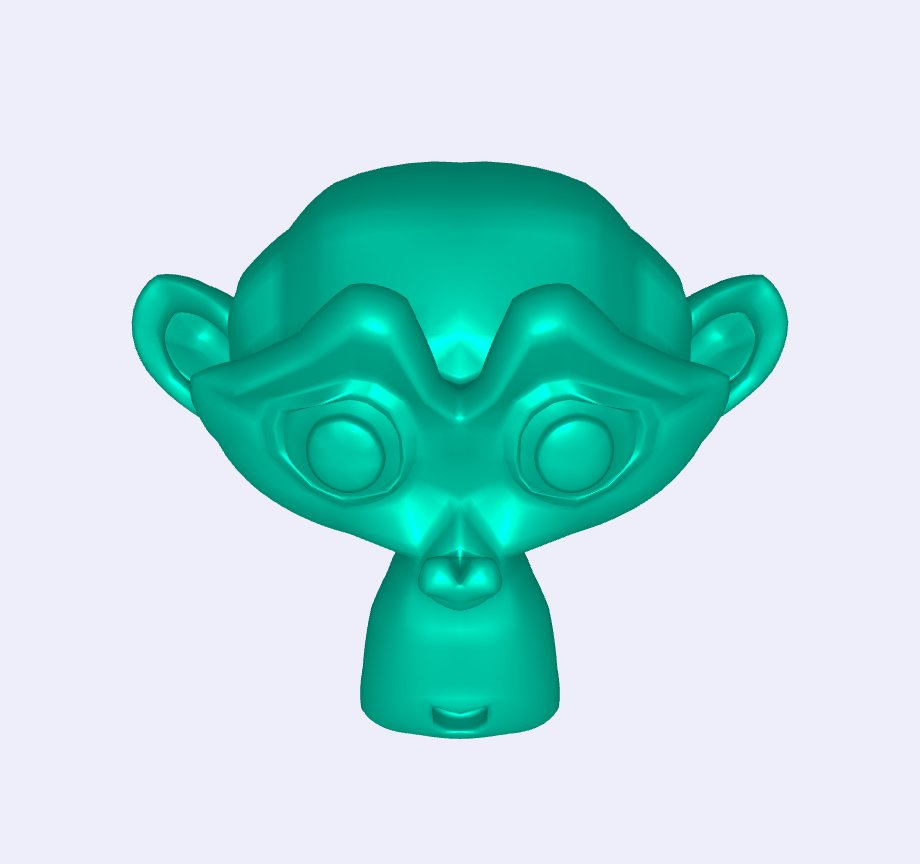
\includegraphics[scale=0.3]{monkey_plastic.png}}
\caption{Model osjenčan difuznom rasvjetom}
\end{center}
\end{figure}

\emph{Difuzno sjenčanje} radi na vrlo jednostavnom principu: intenzitet osnovna boja modela se pojačava, odnosno smanjuje u ovisnosti o kutu koju zatvara zraka svjetlosti i normale plohe na koju ta zraka pada. Kako je prikazano jednadžbom \ref{eq:diffuse}, množenjem matrice normala plohe i matrice pozicije izvora svjetlosti, dobiva se faktor pojačanja. Za konačni rezultat, potrebno je faktor pojačanja pomnožiti sa osnovnom bojom modela.

\begin{equation}
\label{eq:diffuse}
C = (N \cdot L) * B
\end{equation}

Gdje je $N$ matrica normale plohe, $L$ matrica pozicije svijetla te $B$ matrica osnovne boje modela.

\subsection{Cel-shading princip}

\begin{figure}[H]
\label{fig:monkey-toonshaded}
\begin{center}
\fbox{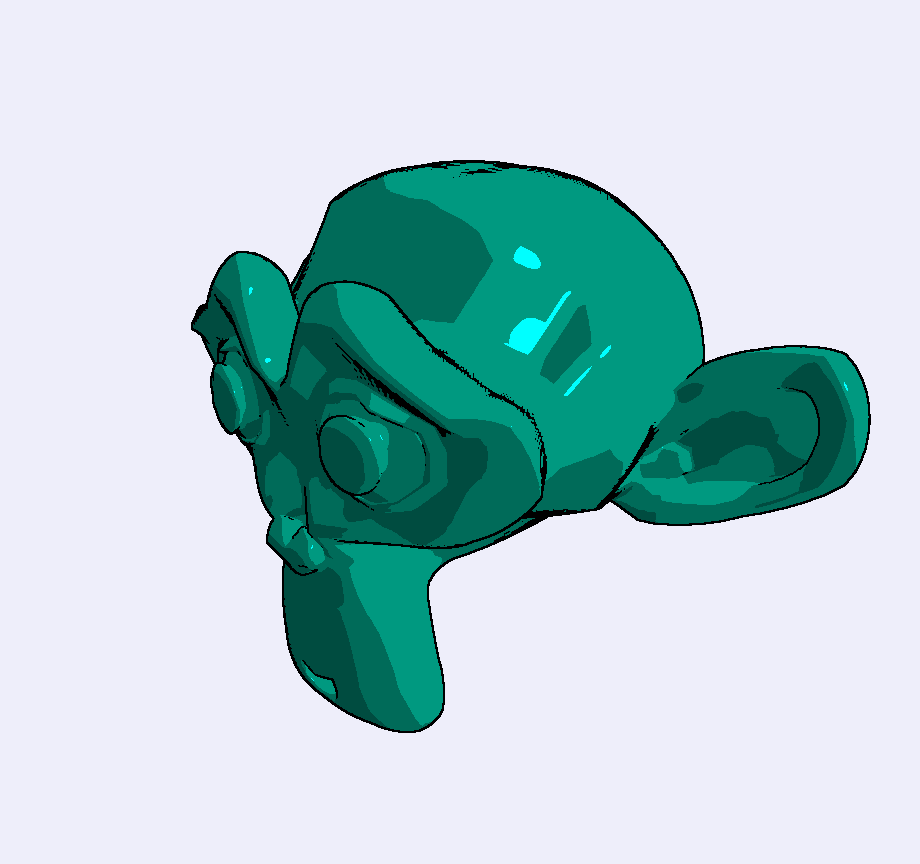
\includegraphics[scale=0.3]{monkey_toonshaded.png}}
\caption{Model osjenčan toon shaderom}
\end{center}
\end{figure}

Što je to uopće i kako se postiže. Koji koraci(slojevi) su potrebni

\subsection{Iscrtavanje obrisa i rubova}

\begin{figure}[H]
\label{fig:monkey-depth}
\begin{center}
\fbox{
\includegraphics[scale=0.3]{monkey_depth.png}}
\caption{Model s iscrtanom \emph{dubinom} pixel-a}
\end{center}
\end{figure}


\begin{figure}[H]
\label{fig:monkey-edges}
\begin{center}
\fbox{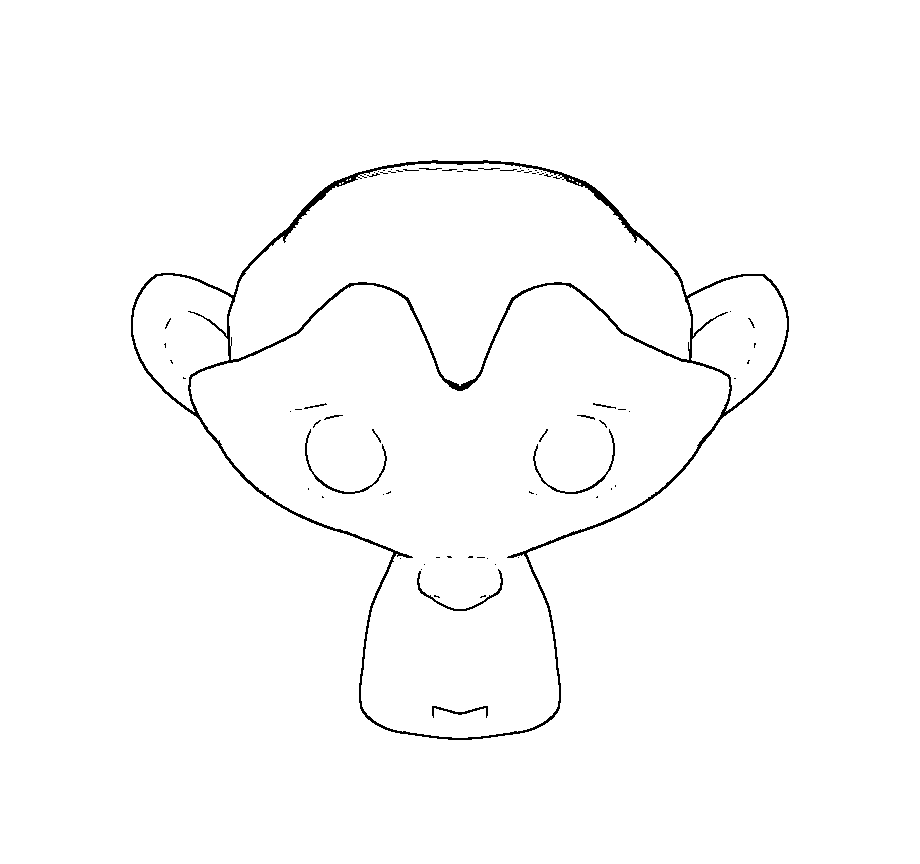
\includegraphics[scale=0.3]{monkey_edges.png}}
\caption{Model s iscrtanim obrisima}
\end{center}
\end{figure}

\subsection{Sjenčanje}

\begin{figure}[H]
\label{fig:monkey-toon}
\begin{center}
\fbox{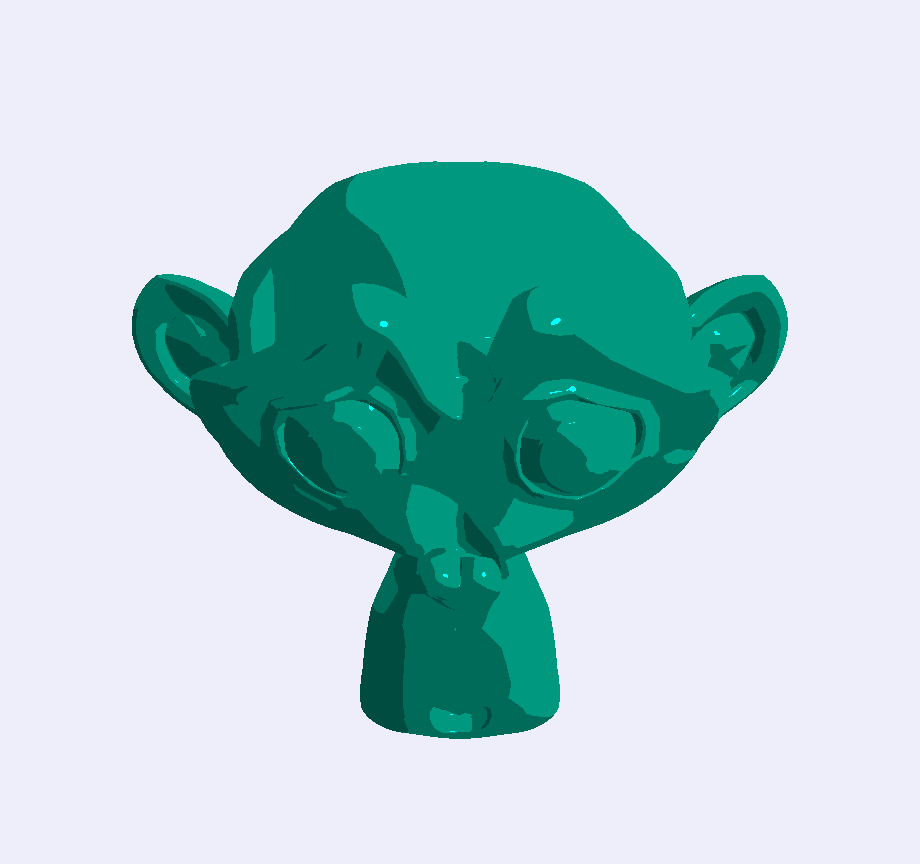
\includegraphics[scale=0.3]{monkey_toon.png}}
\caption{Osjenčani model}
\end{center}
\end{figure}

\subsection{Spajanje slojeva}

\begin{figure}[H]
\label{fig:monkey-final}
\begin{center}
\fbox{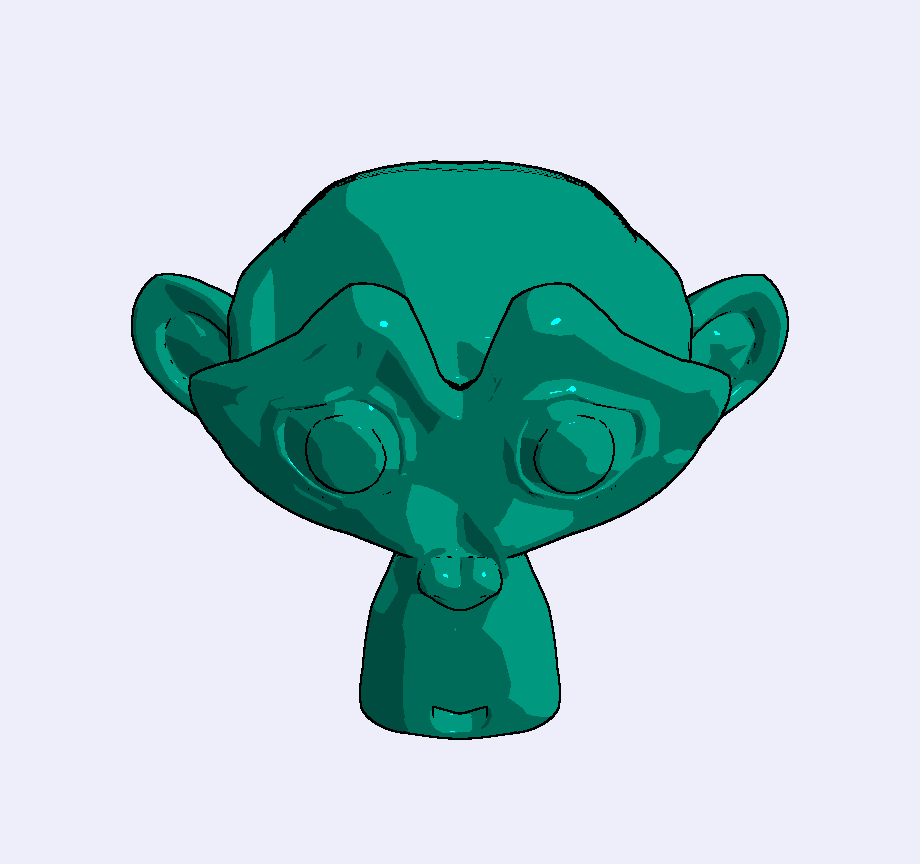
\includegraphics[scale=0.3]{monkey_final.png}}
\caption{Rezultat dobiven spajanjem slojeva}
\end{center}
\end{figure}

Kako se spajaju u cjelinu i što dobijemo s time. Spomenuti ograničenje WebGL-a ovdje